% IEEE conference version for double-blind review, generated from wid_manuscript.tex
% (same text, macros and figures). Every quantitative value is a macro from figures/wid_macros.tex,
% written by code/make_wid_paper.py. Do not type numbers by hand.
\documentclass[conference,a4paper]{IEEEtran}
\IEEEoverridecommandlockouts
\usepackage[T1]{fontenc}
\usepackage{cite}
\usepackage{array}
\usepackage{algorithm}
\usepackage[noend]{algpseudocode}
\usepackage{amsmath,amssymb,booktabs,graphicx,xcolor,microtype}
\usepackage[hidelinks,pdfauthor={},pdfcreator={},pdfproducer={},pdftitle={Soft Biometrics for Writer Identification: A Utility Law from Bangla Handedness}]{hyperref}
% generated by code/make_wid_paper.py from results/wid_handedness_2026-10-29; do not edit by hand
\newcommand{\vnWriters}{42}
\newcommand{\vnLeft}{21}
\newcommand{\vnRight}{21}
\newcommand{\vnImages}{336}
\newcommand{\vnUnits}{5040}
\newcommand{\vnInvalid}{39}
\newcommand{\vnSettings}{120}
\newcommand{\vHandShared}{68.7}
\newcommand{\vHandOwn}{65.5}
\newcommand{\vHandWriter}{73.8}
\newcommand{\vHandStripMin}{61.7}
\newcommand{\vHandStripMax}{66.9}
\newcommand{\vHandAdjOwn}{61.9}
\newcommand{\vHandStrokeOwn}{48.8}
\newcommand{\vStrokeEightOwn}{68.7}
\newcommand{\vScnnFour}{10.7}
\newcommand{\vCrossMin}{44}
\newcommand{\vCrossMax}{53}
\newcommand{\vCrossChance}{51.2}
\newcommand{\vOracleGain}{6.0}
\newcommand{\vOracleMax}{14.9}
\newcommand{\vOracleSig}{106}
\newcommand{\vBayesGain}{$-$0.6}
\newcommand{\vBayesSigUp}{0}
\newcommand{\vBayesSigDown}{1}
\newcommand{\vLoglinGain}{$-$0.2}
\newcommand{\vFilterGain}{$-$14.4}
\newcommand{\vFilterLoss}{14.4}
\newcommand{\vFilterSigDown}{89}
\newcommand{\vPrimDiffMin}{$-$1.5}
\newcommand{\vPrimDiffMax}{$-$0.3}
\newcommand{\vPrimPmin}{0.37}
\newcommand{\vLawR}{0.996}
\newcommand{\vLawMae}{1.5}
\newcommand{\vLawBias}{$-$0.9}
\newcommand{\vLawN}{456}
\newcommand{\vThreshMed}{87}
\newcommand{\vThreshMin}{56}
\newcommand{\vThreshMax}{98}
\newcommand{\vSimAccMin}{60}
\newcommand{\vSimAccMax}{80}
\newcommand{\vSimAccOne}{70}
\newcommand{\vSimGainHiMin}{0.7}
\newcommand{\vSimGainHiMax}{9.8}
\newcommand{\vSimGainObsMax}{2.7}
\newcommand{\vBayesGap}{1.3}
\newcommand{\vGateAcc}{75}
\newcommand{\vGateMin}{$-$8.7}
\newcommand{\vGateMax}{+0.4}
\newcommand{\vPrevLeftNone}{78.6}
\newcommand{\vPrevLeftPriorMin}{2.1}
\newcommand{\vPrevLeftPriorMax}{14.5}
\newcommand{\vPrevBayesLeftMean}{2.7}
\newcommand{\vPrevBayesLeftMax}{14.3}
\newcommand{\vPrevBayesRightLoss}{1.3}
\newcommand{\vLeakHandWI}{65.5}
\newcommand{\vLeakHandEn}{82.1}
\newcommand{\vLeakHandEnShared}{82.1}
\newcommand{\vLeakPseudoWI}{33.3}
\newcommand{\vLeakPseudoEnMin}{52.4}
\newcommand{\vLeakPseudoEnMax}{76.2}
\newcommand{\vLeakPseudoEnShared}{66.4}
\newcommand{\vLeakPseudoEnMean}{62.6}
\newcommand{\vLeakPseudoAbove}{12.6}
\newcommand{\vLeakHandGain}{16.7}
\newcommand{\vLeakGainHandEn}{+1.1}
\newcommand{\vLeakGainPseudoEn}{+0.1}
\newcommand{\vBothGain}{0.95}
\newcommand{\vBothPseudo}{+0.03}
\newcommand{\vBothPseudoScaled}{+0.21}
\newcommand{\vBothPseudoScaledP}{0.048}
\newcommand{\vBothRandom}{+0.19}
\newcommand{\vBothRandomP}{0.010}
\newcommand{\vBothSig}{29}


\begin{document}
\title{Soft Biometrics for Writer Identification: A Utility Law from Bangla Handedness}

% \author{\IEEEauthorblockN{Anonymous Authors}
\IEEEauthorblockA{Affiliation withheld for double-blind review}}

\maketitle

\begin{abstract}
Writer identification from handwriting is a core task of forensic and historical document analysis, and soft biometrics such as handedness are often proposed to narrow its search; whether a \emph{predicted} attribute actually helps, however, has rarely been tested. On the BanglaHand dataset (\vnWriters{} writers), we identified writers from Bangla paragraphs and strips with six representations in \vnSettings{} settings and fused handedness evidence from a model that never saw the queried writer. Known handedness raised top-1 accuracy by \vOracleGain{} points, because identification errors were unrelated to hand. Predicted handedness (\vHandOwn\% accurate) did not help: Bayesian fusion changed top-1 by \vBayesGain{} points and gallery filtering by \vFilterGain{}. A utility law, top-1 with filtering = attribute accuracy $\times$ top-1 with known attribute, matched all \vLawN{} cases ($r=\vLawR$) and implies that filtering needs about \vThreshMed\% accuracy, and a random-label control showed that attribute accuracy obtained on enrolled writers mainly measures writer recognition. The study gives the community a simple test of when a soft biometric is worth fusing with identification and a cheap check for leakage in reported attribute accuracies, the first such evidence for Bangla handwriting.
\end{abstract}

\begin{IEEEkeywords}
Writer identification, Soft biometrics, Handedness, Bangla handwriting, Score fusion, Data leakage
\end{IEEEkeywords}

\section{Introduction}
Soft biometric traits such as gender, age or handedness do not identify a person, but they can complement a primary biometric by excluding candidates or reweighting scores \cite{jain2004soft,dantcheva2016soft}. In handwriting, gender and handedness have been predicted from offline samples \cite{liwicki2011gender,siddiqi2015gender,hassaine2013icdar,bouadjenek2016soft,almaadeed2016handedness,morera2018handedness,rahmanian2021handedness}, often with the aim of narrowing the search of writer identification \cite{banglahand2026dataset}. Whether this works depends on two numbers that are rarely reported together: how accurately the attribute is predicted for writers the model has never seen, and how often identification errors cross the attribute boundary. In forensic examination of Bangla documents, for example, a suspect's handedness may be known from the investigation, whereas that of the writer of a questioned document must be inferred from the handwriting itself.

A second problem is leakage. Handwriting identifies its writer very well \cite{bulacu2007text,schomaker2007codebooks}, so an attribute model trained on samples of the same writers it is applied to can recognise the writer and inherit the label \cite{kaufman2012leakage}. In closed-set identification, where all gallery writers are known, this design is tempting.

We study both questions for handedness in Bangla, using a balanced, acquisition-controlled dataset \cite{banglahand2026dataset} for which writer-independent handedness prediction has been characterised \cite{anon2026handedness}. The contributions are: (i) a closed-set identification study with known and predicted handedness in \vnSettings{} settings; (ii) a utility law that predicts the effect of attribute filtering from attribute accuracy, and the accuracy at which Bayesian fusion starts to help; (iii) a random-label control that separates attribute information from writer identity; and (iv) consequences for gallery prevalence and for the reporting of soft-biometric accuracies. Fig.~\ref{fig:method} summarises the procedure.

\section{Related work}
\label{sec:related}
Soft traits were proposed as auxiliary evidence for a primary biometric in personal recognition \cite{jain2004soft}, and a survey covers their extraction from many modalities \cite{dantcheva2016soft}.

Gender has been predicted from on-line and off-line handwriting \cite{liwicki2011gender,siddiqi2015gender}, in an ICDAR 2013 competition with 194 participating teams \cite{hassaine2013icdar}, and together with other soft biometrics \cite{bouadjenek2016soft}. Handedness was predicted from Arabic and English texts of 121 writers with fuzzy feature reduction and a $k$-nearest-neighbour classifier \cite{almaadeed2016handedness}, and with convolutional networks on the IAM and KHATT collections \cite{morera2018handedness} and in later work \cite{rahmanian2021handedness}. Reported handedness accuracies range from F-measures of about 70\% \cite{almaadeed2016handedness} to above 99\% \cite{rahmanian2021handedness}, under protocols that differ in whether test writers were seen in training \cite{anon2026handedness}. These studies report attribute accuracy only.

Text-independent writer identification describes a writer by distributions of contour directions, hinges and graphemes \cite{bulacu2007text} or by codebooks of contour fragments \cite{schomaker2007codebooks}. For Bangla, public collections support writer identification (BanglaWriting, 260 writers) \cite{mridha2021banglawriting} and character recognition (Boise State, 100 writers) \cite{majid2018bangla}, and writer verification reached 94.54\% for 100 writers \cite{paul2024bangla}. Table~\ref{tab:related} summarises these works; none of the handwriting studies measured how a known or predicted attribute changes identification.

\begin{table*}[t]
\caption{Related work. Writers: number of writers stated in the cited abstract or record; --: not stated there. G: gender, H: handedness, SB: several soft biometrics.}
\label{tab:related}
\centering\scriptsize
\setlength{\tabcolsep}{3pt}
\begin{tabular}{l>{\raggedright\arraybackslash}p{2.7cm}>{\raggedright\arraybackslash}p{3.1cm}c>{\raggedright\arraybackslash}p{3.4cm}>{\raggedright\arraybackslash}p{2.3cm}}
\toprule
Work & Task & Script / data & Writers & Method & Reported result \\
\midrule
Jain et al.\ \cite{jain2004soft} & soft traits in personal recognition & primary biometric + soft traits & -- & fusion with primary biometric & -- \\
Liwicki et al.\ \cite{liwicki2011gender} & G & on-line and off-line handwriting & -- & on-line and off-line features & -- \\
Hassa\"ine et al.\ \cite{hassaine2013icdar} & G (competition) & competition data (Kaggle) & -- & 194 participating teams & -- \\
Siddiqi et al.\ \cite{siddiqi2015gender} & G & off-line handwriting & -- & handwriting features & -- \\
Bouadjenek et al.\ \cite{bouadjenek2016soft} & SB & off-line handwriting & -- & -- & -- \\
Al-Maadeed et al.\ \cite{almaadeed2016handedness} & H & Arabic, English & 121 & fuzzy feature reduction, $k$-NN & F-measure about 70\% \\
Morera et al.\ \cite{morera2018handedness} & G, H, G+H & English (IAM), Arabic (KHATT) & -- & CNN & -- \\
Rahmanian and Shayegan \cite{rahmanian2021handedness} & G, H & -- & -- & CNN & above 99\% \\
Bulacu and Schomaker \cite{bulacu2007text} & writer identification & off-line, text-independent & -- & contour-direction, hinge, grapheme PDFs & -- \\
Schomaker et al.\ \cite{schomaker2007codebooks} & writer identification & forensic and historic documents & -- & contour-fragment codebooks & -- \\
Mridha et al.\ \cite{mridha2021banglawriting} & dataset (writer ID, OCR) & Bangla (BanglaWriting) & 260 & -- & -- \\
Majid and Barney Smith \cite{majid2018bangla} & dataset, character recognition & Bangla (Boise State) & 100 & bag of features, SVM & 95.4\% characters \\
Paul et al.\ \cite{paul2024bangla} & writer verification & Bangla & 100 & handcrafted features, genetic selection & 94.54\% verification \\
\cite{anon2026handedness} & H, writer-independent & Bangla (BanglaHand) & 42 & gradient descriptor, linear SVM & 77.4\% writer balanced acc. \\
\bottomrule
\end{tabular}
\end{table*}

\begin{figure*}[t]
\centering
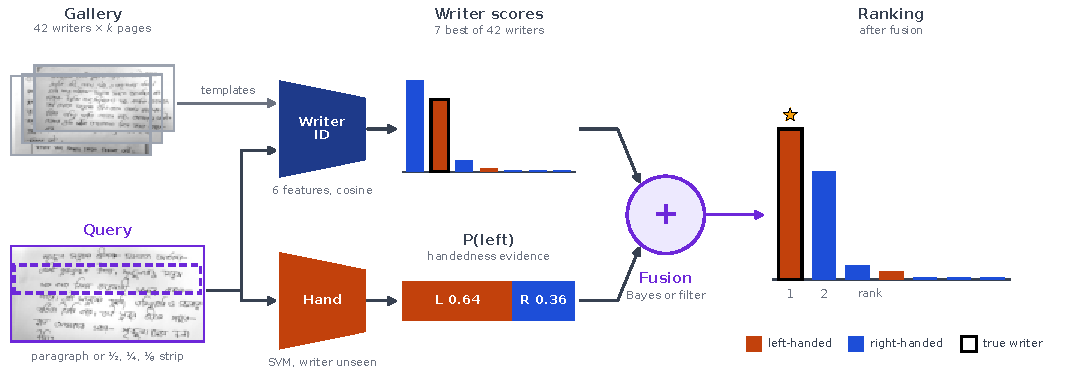
\includegraphics[width=\textwidth]{figures/fig0_method.pdf}
\caption{Procedure for one real query (ViT-B/16, own-text paragraph, six references). The query, a paragraph or a strip (dashed: one of four), is scored against all 42 gallery writers (Writer ID; orange left-, blue right-handed, outlined the true writer) and given a probability of left-handedness by a model that never saw this writer (Hand); fusion combines both. Here the true writer (star) moved from rank 2 to rank 1; on average, fusion did not help (Section~\ref{sec:pred}).}
\label{fig:method}
\end{figure*}

\section{Data and identification}
\label{sec:data}
BanglaHand \cite{banglahand2026dataset} contains \vnImages{} smartphone photographs of paragraphs by \vnWriters{} writers (\vnLeft{} left-, \vnRight{} right-handed); each wrote six shared prompts (paragraphs 1--6) and two texts of their own choice (7--8) with shared materials, photographed in one session. Each paragraph is a \emph{unit} ($n=1$) and is also cut into $n=2$, 4 or 8 horizontal strips of about 3.5, 1.75 and 0.9 lines (Fig.~\ref{fig:method}): the text block is divided into equal bands and each cut is moved to the emptiest row of the smoothed ink profile within half a line pitch. Strips keep the full width, and hence the scale, of the photograph. Of \vnUnits{} units, \vnInvalid{} strips with too little writing were removed.

Six representations from \cite{anon2026handedness} are computed on every unit: writing-only STROKE features (208 contour-direction, hinge, curvature, stroke-ending and slant histograms), the HC-183 gradient descriptor of the ink mask, frozen ImageNet ResNet-18 \cite{he2016resnet}, EfficientNet-B0 \cite{tan2019efficientnet} and ViT-B/16 \cite{dosovitskiy2021vit} embeddings of grey tiles, and Stroke-CNN (ResNet-18 on binary ink tiles). For whole paragraphs they equal those of \cite{anon2026handedness}.

Identification is closed-set over all \vnWriters{} writers. Features are standardised without labels and L2-normalised; a writer's template is the mean of $k$ whole shared paragraphs, and the score $s_w$ is the cosine similarity. Shared queries are matched against the other five prompts of every writer ($k=5$), own-text queries against every subset of $k=1$, 2, 3 or 6 prompts. Four query sizes, five reference conditions and six representations give \vnSettings{} settings; the endpoint is top-1 accuracy, averaged over reference subsets.

\section{Handedness evidence and fusion}
\label{sec:methods}
For every writer, a linear SVM ($C=0.1$, as in \cite{anon2026handedness}) on HC-183 is trained on shared units of the same size $n$ from the other 41 writers and scores all units of the held-out writer; Platt scaling \cite{platt1999probabilistic}, fitted by inner five-fold cross-validation over the training writers, turns the scores into a log-odds $\ell$ of left-handedness. Sensitivity analyses use STROKE, HC-183 with ink density and photo intensity regressed out \cite{anon2026handedness}, or $\ell$ averaged over all own-text units of a writer.

Three scenarios are compared: \emph{known}, with both hands known (for example, a suspect's hand known from the investigation); \emph{query} (primary), with gallery hands known and the query hand predicted; and \emph{both}, with gallery hands also predicted from the writer's references. With $P(h\mid x)=\sigma(\pm\ell)$, \emph{Bayes} fusion ranks writers by $\log\mathrm{softmax}_w(s_w/T)+\log P(h_w\mid x)$, where $h_w$ is the hand of writer $w$; \emph{log-linear} fusion weights the second term by $\lambda$; and the \emph{filter} ranks writers of the predicted hand first. $T$ and $\lambda$ are fitted on the queries of the other writers only. Algorithm~\ref{alg:eval} summarises one evaluation.
\begin{algorithm}[t]
\caption{Evaluation of one setting with predicted query handedness}
\label{alg:eval}
\footnotesize
\begin{algorithmic}[1]
\Require unit features, writer identities, hands $h_v$ of the 42 writers, reference sets $\mathcal{R}$
\For{each writer $w$}
  \State train the SVM on shared units (size $n$) of all writers $v\neq w$
  \State fit Platt scaling by inner five-fold cross-validation over them
  \State $\ell_u\gets$ calibrated left-handed log-odds of every unit $u$ of $w$
\EndFor
\For{each reference set $R\in\mathcal{R}$ and query unit $q$}
  \State $t_v\gets$ mean normalised features of $R$ for every writer $v$
  \State $s_v\gets\cos(x_q,t_v)$ for all writers $v$
\EndFor
\For{each writer $w$}
  \State fit $T$ on the queries of writers $v\neq w$ (minimum NLL)
  \State rank writers by $\log\mathrm{softmax}_v(s_v/T)+\log P(h_v\mid\ell_q)$ for every query $q$ of $w$
\EndFor
\State \Return top-1 per query; writer-level difference to no fusion
\end{algorithmic}
\end{algorithm}


If the hand is predicted correctly with probability $a$, independently of identification, filtering keeps the true writer with probability $a$ and then succeeds as often as with known hands:
\begin{equation}
\mathrm{top1}_{\mathrm{filter}} = a \cdot \mathrm{top1}_{\mathrm{known}},
\label{eq:law}
\end{equation}
so filtering helps only if $a > \mathrm{top1}_{\mathrm{none}}/\mathrm{top1}_{\mathrm{known}}$. In words, a filter whose hand prediction is right 70\% of the time discards the true writer in 30\% of queries, and it pays off only if knowing the hand gains more than that loss. Bayesian fusion has no closed form, so we replaced $\ell$ by synthetic calibrated evidence of accuracy $a=0.50,\dots,1.00$ (equal-variance Gaussian scores, log-odds $d\,z$ with $d=2\Phi^{-1}(a)$; 200 draws). Prevalence was studied with galleries of the \vnRight{} right-handed and $m=1$, 2 or 3 left-handed writers (1,000 draws), where the prior decision rule calls a query left-handed if $\ell+\log(m/\vnRight)>0$.

For the leakage control, the SVM was also trained on the enrolled writers themselves (\emph{enrolment-trained}): shared units were scored by five-fold cross-validation over paragraphs, so other paragraphs of the same writer were in training, and own-text units by the model fitted on all shared units. Both regimes were repeated with 20 random 21/21 writer splits as labels, each balanced for hand, so that accuracy and identification gain reached by a random label measure writer identity. The \emph{both} scenario was controlled the same way and with random directions of HC-183 scaled to the spread of $\ell$.

Differences in top-1 are computed per writer and tested with 9,999 sign flips over writers, with 2,000 writer-bootstrap intervals stratified by hand. Four primary tests, specified in advance, compare Bayes fusion (query scenario) with no fusion for ResNet-18 and ViT-B/16 on own-text paragraphs with one reference and on quarter strips with six references (Holm correction); all other $p$-values, and counts of significant settings, which share writers, are descriptive. A feasibility check on saved paragraph features, which covered the paragraph-level primary settings, preceded the protocol.

\section{Results}
\subsection{Known handedness complements identification}
Writer-independent handedness was predicted with \vHandShared\% unit accuracy on shared paragraphs, \vHandOwn\% on own texts and \vHandWriter\% at the writer level, and with \vHandStripMin--\vHandStripMax\% on strips; adjusted HC-183 (\vHandAdjOwn\%) and STROKE (\vHandStrokeOwn\%) were weaker (Table~\ref{tab:hand}). No model or query size came close to the break-even accuracies of Section~\ref{sec:law}.
\begin{table}[t]
\caption{Writer-independent handedness accuracy (\%, shared / own-text units) by query size, and writer-level accuracy (paragraph units averaged per writer). Linear SVM, leave one writer out.}
\label{tab:hand}
\centering\scriptsize
\setlength{\tabcolsep}{3pt}
\begin{tabular}{lccccc}
\toprule
Model & Paragraph & $\frac{1}{2}$ strip & $\frac{1}{4}$ strip & $\frac{1}{8}$ strip & Writer \\
\midrule
% generated by code/make_wid_paper.py
HC-183 & 68.7 / 65.5 & 65.9 / 66.1 & 65.9 / 66.9 & 63.2 / 61.7 & 73.8 \\
HC-183 adj. & 56.7 / 61.9 & 63.3 / 57.1 & 58.6 / 60.9 & 60.8 / 59.3 & 61.9 \\
STROKE & 53.2 / 48.8 & 51.6 / 46.4 & 44.6 / 41.2 & 46.6 / 46.7 & 54.8 \\
\bottomrule
% ends with \bottomrule
\end{tabular}
\end{table}
 Among identification features, STROKE was strongest (\vStrokeEightOwn\% top-1 on one-line own-text strips with one reference), while Stroke-CNN collapsed on strips (\vScnnFour\% at $n=4$).

Identification errors were unrelated to hand: \vCrossMin--\vCrossMax\% of misidentified queries went to a writer of the other hand, against \vCrossChance\% expected by chance (Fig.~\ref{fig:query}c). Known handedness therefore removed about half of the competitors and raised top-1 by \vOracleGain{} points on average (up to \vOracleMax), significantly in \vOracleSig{} of \vnSettings{} settings (Table~\ref{tab:main}). Accuracy fell as the query shrank and rose with more reference pages, and the gain from a known hand was largest where identification was weakest, whereas fusion with the predicted hand stayed at or below the baseline throughout (Fig.~\ref{fig:query}a,b).

\begin{figure*}[t]
\centering
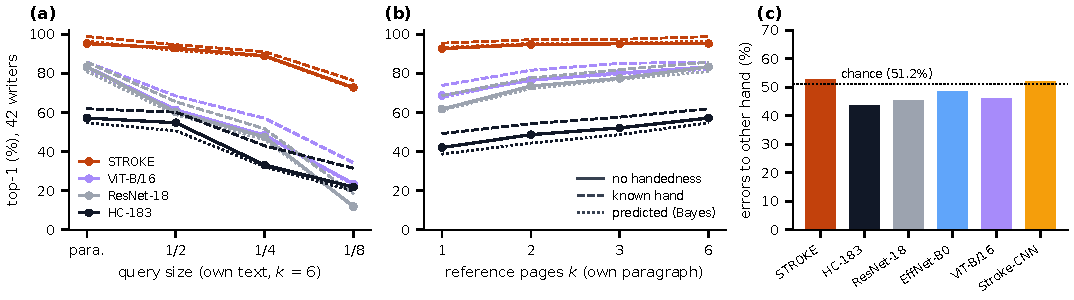
\includegraphics[width=\textwidth]{figures/fig_query.pdf}
\caption{Identification with and without handedness. Top-1 accuracy (a) as the own-text query shrinks from a paragraph to about one line (six references) and (b) as the number of reference pages grows (own-text paragraph queries): no handedness (solid), known hand (dashed), predicted hand with Bayes fusion (dotted). (c) Share of identification errors whose top-ranked writer has the other hand, over all settings of each representation; dotted: share expected if errors were unrelated to hand.}
\label{fig:query}
\end{figure*}

\begin{table*}[t]
\caption{Top-1 identification accuracy (\%) without handedness (None), with known handedness (Known) and with predicted query handedness (Bayes fusion; filter): own-text paragraph against one shared reference (mean over the six choices), own-text quarter strip against six references, and shared quarter strip against the other five prompts. Handedness: HC-183, leave one writer out.}
\label{tab:main}
\centering\footnotesize
\begin{tabular}{lcccccccccccc}
\toprule
 & \multicolumn{4}{c}{Own paragraph, $k=1$} & \multicolumn{4}{c}{Own quarter strip, $k=6$} & \multicolumn{4}{c}{Shared quarter strip, $k=5$} \\
\cmidrule(lr){2-5}\cmidrule(lr){6-9}\cmidrule(lr){10-13}
Representation & None & Known & Bayes & Filter & None & Known & Bayes & Filter & None & Known & Bayes & Filter \\
\midrule
% generated by code/make_wid_paper.py
STROKE & 92.7 & 95.4 & 93.3 & 62.1 & 89.0 & 91.0 & 88.7 & 60.0 & 96.0 & 96.9 & 95.7 & 63.7 \\
HC-183 & 42.1 & 49.2 & 38.7 & 28.0 & 33.1 & 43.0 & 32.2 & 25.7 & 42.4 & 52.1 & 41.1 & 34.2 \\
ResNet-18 & 61.7 & 68.7 & 61.1 & 42.9 & 47.5 & 51.6 & 46.0 & 35.8 & 63.4 & 69.7 & 62.7 & 45.7 \\
EffNet-B0 & 55.6 & 62.5 & 53.8 & 38.7 & 49.3 & 57.6 & 49.0 & 38.2 & 63.7 & 70.5 & 63.5 & 45.0 \\
ViT-B/16 & 68.7 & 73.8 & 67.5 & 45.2 & 48.4 & 57.0 & 48.1 & 39.1 & 64.8 & 72.2 & 64.7 & 45.8 \\
Stroke-CNN & 58.9 & 70.6 & 60.1 & 43.8 & 10.7 & 15.5 & 10.7 & 8.4 & 15.8 & 23.9 & 16.6 & 14.3 \\
\bottomrule
% ends with \bottomrule
\end{tabular}
\end{table*}

\subsection{Predicted handedness does not help}
\label{sec:pred}
None of the four primary tests showed a gain (differences \vPrimDiffMin{} to \vPrimDiffMax{} points, $p\geq\vPrimPmin$, Holm $p=1$; Table~\ref{tab:tests}). Over all settings, Bayes fusion changed top-1 by \vBayesGain{} points on average (significant gains in \vBayesSigUp{}, losses in \vBayesSigDown{} settings), log-linear fusion by \vLoglinGain{}, as its weight was fitted near zero, and the filter by \vFilterGain{} points (losses in \vFilterSigDown{} settings).

\begin{table}[t]
\caption{Primary tests: Bayes fusion of predicted query handedness against no fusion (top-1, \%). Diff.: writer-level mean difference (points) with writer-bootstrap interval; $p$: 9,999 sign flips; Holm over the four tests.}
\label{tab:tests}
\centering\scriptsize
\setlength{\tabcolsep}{1.8pt}
\resizebox{\columnwidth}{!}{%
\begin{tabular}{llccccc}
\toprule
Setting & Representation & None & Bayes & Diff. [95\% CI] & $p$ & Holm \\
\midrule
% generated by code/make_wid_paper.py
Own paragraph, $k=1$ & ResNet-18 & 61.7 & 61.1 & $-$0.6 [$-$4.0, +2.2] & 0.84 & 1.00 \\
Own paragraph, $k=1$ & ViT-B/16 & 68.7 & 67.5 & $-$1.2 [$-$3.6, +1.2] & 0.48 & 1.00 \\
Own strip ($n=4$), $k=6$ & ResNet-18 & 47.5 & 46.0 & $-$1.5 [$-$4.2, +0.9] & 0.37 & 1.00 \\
Own strip ($n=4$), $k=6$ & ViT-B/16 & 48.4 & 48.1 & $-$0.3 [$-$3.6, +2.7] & 1.00 & 1.00 \\
\bottomrule
% ends with \bottomrule
\end{tabular}}
\end{table}

\subsection{A utility law}
\label{sec:law}
Eq.~\eqref{eq:law} predicted the filter accuracy of all \vLawN{} combinations of setting and handedness model ($r=\vLawR$, mean absolute error \vLawMae{} points, bias \vLawBias; Fig.~\ref{fig:utility}a). The break-even accuracy for own-text queries was \vThreshMed\% (median; range \vThreshMin--\vThreshMax\%), far above the \vHandOwn\% achieved. With synthetic calibrated evidence (Fig.~\ref{fig:utility}b), Bayes fusion gained at least half a point from an accuracy of \vSimAccMin--\vSimAccMax\%, at most \vSimGainObsMax{} points at the achieved accuracy, and \vSimGainHiMin--\vSimGainHiMax{} points at 95\%. The real evidence fell \vBayesGap{} points short of synthetic evidence of equal accuracy, so it is less well calibrated or not independent of identification. Applying the filter only to the most confident 30\% of predictions (\vGateAcc\% accurate, still below break-even) changed top-1 by \vGateMin{} to \vGateMax{} points.

\begin{figure*}[t]
\centering
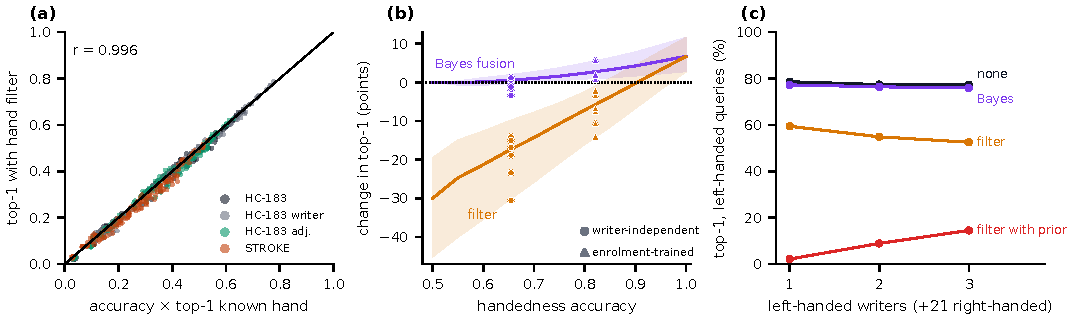
\includegraphics[width=\textwidth]{figures/fig2_utility.pdf}
\caption{(a) Utility law: observed top-1 with hand filtering against handedness accuracy $\times$ top-1 with known handedness (Eq.~\ref{eq:law}), for every setting and handedness model. (b) Change in top-1 against handedness accuracy for synthetic calibrated evidence (lines: mean over representations; band: range; own-text paragraphs, one reference) and for real evidence (circles: writer-independent; triangles: enrolment-trained). (c) Galleries of \vnRight{} right-handed and 1--3 left-handed writers: top-1 of left-handed queries (ViT-B/16, own-text paragraphs, one reference).}
\label{fig:utility}
\end{figure*}

When left-handed writers were rare (one to three in the gallery; Fig.~\ref{fig:utility}c), Bayes fusion raised top-1 of left-handed queries by \vPrevBayesLeftMean{} points on average (up to \vPrevBayesLeftMax{} for weak representations) and lowered that of right-handed queries by at most \vPrevBayesRightLoss{}. A filter using the prior decision rule, however, lowered top-1 of left-handed queries (ViT-B/16) from \vPrevLeftNone\% to \vPrevLeftPriorMin--\vPrevLeftPriorMax\%: an attribute model of this accuracy cannot overcome a low prior.

\subsection{Leakage control}
Trained on the enrolled writers, the handedness model reached \vLeakHandEn\% on own-text paragraphs, \vLeakHandGain{} points more than for unseen writers (\vLeakHandWI\%; Fig.~\ref{fig:leak}a). Random labels reached \vLeakPseudoEnMin--\vLeakPseudoEnMax\% (mean \vLeakPseudoEnMean\%, \vLeakPseudoAbove{} points above chance) under the same training, but fell below chance for unseen writers (\vLeakPseudoWI\%), the known bias of leave-one-out on uninformative labels. Most of the accuracy gained by enrolment training therefore reflects the writer, not the hand. In identification (Fig.~\ref{fig:leak}b), enrolment-trained handedness changed top-1 by \vLeakGainHandEn{} points and random labels by \vLeakGainPseudoEn.

\begin{figure*}[t]
\centering
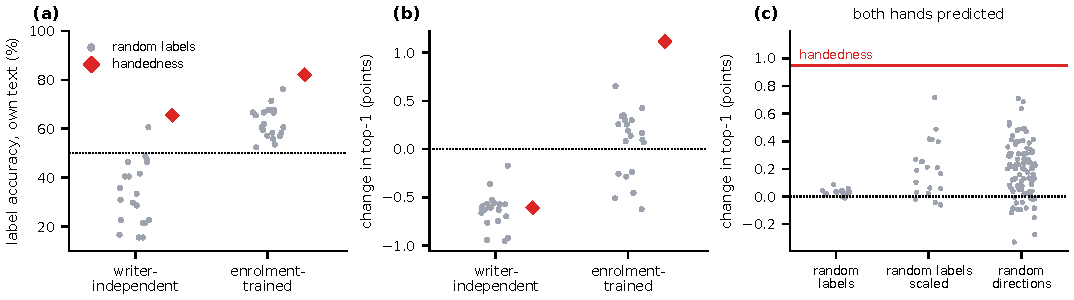
\includegraphics[width=\textwidth]{figures/fig3_leakage.pdf}
\caption{Random-label control. (a) Accuracy on own-text paragraphs of handedness (red) and of 20 random hand-balanced labels (grey), for models that never saw the writer (writer-independent) or were trained on the enrolled writers. (b) Mean change in top-1 over all settings with this evidence fused (Bayes, gallery labels known). (c) Scenario \emph{both}: mean change in top-1 with handedness evidence, random labels (calibrated, or scaled to the spread of the handedness log-odds) and random directions of HC-183.}
\label{fig:leak}
\end{figure*}

\subsection{Predicted hands on both sides}
In an exploratory analysis with gallery hands also predicted, fusion raised top-1 by \vBothGain{} points on average (significant in \vBothSig{} settings, never lower). Random labels changed top-1 by \vBothPseudo{} points, scaled random labels by \vBothPseudoScaled{} ($p=\vBothPseudoScaledP$) and random directions by \vBothRandom{} ($p=\vBothRandomP$; Fig.~\ref{fig:leak}c). Agreement of predicted hands thus adds a little information that random projections do not, best read as agreement on a writer-consistent, handedness-related trait.

\subsection{Comparison with previous work}
Table~\ref{tab:compare} compares the scope of this study with earlier work. Earlier studies either predicted attributes \cite{liwicki2011gender,siddiqi2015gender,hassaine2013icdar,bouadjenek2016soft,almaadeed2016handedness,morera2018handedness,rahmanian2021handedness} or identified writers without them \cite{bulacu2007text,schomaker2007codebooks,paul2024bangla}. To our knowledge, this is the first study to address all columns of the table, and the first for Bangla.

\begin{table*}[t]
\caption{Comparison with previous work. \checkmark: addressed; $\times$: not addressed according to the cited title and abstract; --: not applicable or not stated. Attr.\ to ID: attribute used to change writer identification; Known/pred.: known and predicted attribute compared; Break-even: attribute accuracy at which fusion helps; Random labels: control for writer identity in attribute accuracy; Prev.: attribute prevalence in the gallery; Acq.: acquisition-controlled data. G: gender, H: handedness, SB: several soft biometrics.}
\label{tab:compare}
\centering\scriptsize
\setlength{\tabcolsep}{2.6pt}
\begin{tabular}{l>{\raggedright\arraybackslash}p{1.45cm}cccccccccc>{\raggedright\arraybackslash}p{4.2cm}}
\toprule
Work & Script & Writers & Attr. & \shortstack{Writer\\ID} & \shortstack{Attr.\\to ID} & \shortstack{Known/\\pred.} & \shortstack{Break-\\even} & \shortstack{Random\\labels} & Prev. & Acq. & Key result \\
\midrule
\cite{jain2004soft} & -- & -- & SB & \checkmark & \checkmark & -- & -- & -- & -- & -- & -- \\
\cite{liwicki2011gender} & -- & -- & G & $\times$ & $\times$ & $\times$ & $\times$ & $\times$ & $\times$ & -- & -- \\
\cite{hassaine2013icdar} & -- & -- & G & $\times$ & $\times$ & $\times$ & $\times$ & $\times$ & $\times$ & -- & competition, 194 teams \\
\cite{siddiqi2015gender} & -- & -- & G & $\times$ & $\times$ & $\times$ & $\times$ & $\times$ & $\times$ & -- & -- \\
\cite{bouadjenek2016soft} & -- & -- & SB & $\times$ & $\times$ & $\times$ & $\times$ & $\times$ & $\times$ & -- & -- \\
\cite{almaadeed2016handedness} & Arabic, English & 121 & H & $\times$ & $\times$ & $\times$ & $\times$ & $\times$ & $\times$ & -- & F-measure about 70\% \\
\cite{morera2018handedness} & English, Arabic & -- & G, H & $\times$ & $\times$ & $\times$ & $\times$ & $\times$ & $\times$ & -- & -- \\
\cite{rahmanian2021handedness} & -- & -- & G, H & $\times$ & $\times$ & $\times$ & $\times$ & $\times$ & $\times$ & -- & above 99\% \\
\cite{bulacu2007text} & -- & -- & -- & \checkmark & $\times$ & -- & -- & -- & -- & -- & -- \\
\cite{paul2024bangla} & Bangla & 100 & -- & \checkmark & $\times$ & -- & -- & -- & -- & -- & 94.54\% verification \\
\cite{anon2026handedness} & Bangla & 42 & H & \checkmark & $\times$ & $\times$ & $\times$ & $\times$ & $\times$ & \checkmark & 77.4\% writer bal.\ acc. \\
This work & Bangla & \vnWriters & H & \checkmark & \checkmark & \checkmark & \checkmark & \checkmark & \checkmark & \checkmark & known $+$\vOracleGain, predicted \vBayesGain{} points; filter needs \vThreshMed\% \\
\bottomrule
\end{tabular}
\end{table*}

\section{Discussion}
\label{sec:disc}
Handedness is complementary to writer identification: features from contour hinges to ImageNet embeddings made errors unrelated to hand, so a known hand removes half of the competitors. The value of a predicted hand is set by Eq.~\eqref{eq:law}: filtering needs about \vThreshMed\% accuracy and Bayesian fusion about \vSimAccOne\% for a one-point gain, whereas writer-independent handedness from offline Bangla handwriting reaches \vHandOwn--\vHandWriter\% here and 77\% balanced accuracy in \cite{anon2026handedness}. Predicted handedness should therefore not filter galleries and should be fused only as a calibrated probability, which gives a rare minority class a small gain at little cost; known handedness is worth using in casework.

The random-label control shows why high attribute accuracies are easy to obtain and misleading: trained on the enrolled writers, a meaningless label reached up to \vLeakPseudoEnMax\%, more than real handedness for unseen writers. Soft-biometric studies should state whether test writers were seen in training, and a random-label run is a cheap check. Eq.~\eqref{eq:law} needs only two accuracies, so it can be applied to other attributes before any fusion experiment.

Identification used frozen and handcrafted features by design, as \vnWriters{} writers are too few to train identification networks without a risk of overfitting. The main limitation is sample size, set by availability: left-handed writers are rare and left-hand use is culturally discouraged in many regions \cite{papadatou2020handedness}, so the balanced collection has \vnWriters{} writers from one region and one phone. No other Bangla collection with handedness labels exists for replication, offline photographs cannot record pen pressure or stroke order, and per-writer gender is not in the metadata, so only one real attribute could be tested.

\section{Conclusion}
On \vnWriters{} Bangla writers, known handedness raised writer identification accuracy by \vOracleGain{} points, whereas handedness predicted for unseen writers (\vHandOwn\% accurate) did not help and gallery filtering cost \vFilterLoss{} points. A utility law predicted these results, and a random-label control showed that attribute accuracies obtained on enrolled writers mainly reflect writer identity. Soft biometrics should be fused with identification only when they are known or predicted far more accurately than offline handwriting currently allows. Future work will test Eq.~\eqref{eq:law} on further attributes, such as gender, and on larger collections in other scripts, and will try to raise writer-independent handedness accuracy towards the break-even point, for example with more text per questioned document or with pen-pressure and on-line stroke cues.

\section*{Data and code availability}
The BanglaHand dataset is publicly available under a CC BY 4.0 licence \cite{banglahand2026dataset}. The analysis code and saved results will be released upon acceptance.

\section*{Ethics statement}
Informed consent was obtained voluntarily from all participants prior to data collection. No personal identifying information was collected, and all handwriting samples are pseudonymous.

\bibliographystyle{IEEEtran}
\bibliography{references}
\end{document}
